\documentclass[a3paper]{article}
\usepackage[T1]{fontenc}
\usepackage{lmodern}
\usepackage{amssymb,amsmath}
\usepackage{ifxetex,ifluatex}
\usepackage{fixltx2e} % provides \textsubscript
% use upquote if available, for straight quotes in verbatim environments
\IfFileExists{upquote.sty}{\usepackage{upquote}}{}
\ifnum 0\ifxetex 1\fi\ifluatex 1\fi=0 % if pdftex
  \usepackage[utf8]{inputenc}
\else % if luatex or xelatex
  \ifxetex
    \usepackage{mathspec}
    \usepackage{xltxtra,xunicode}
  \else
    \usepackage{fontspec}
  \fi
  \defaultfontfeatures{Mapping=tex-text,Scale=MatchLowercase}
  \newcommand{\euro}{€}
\fi
% use microtype if available
\IfFileExists{microtype.sty}{\usepackage{microtype}}{}
\usepackage[margin=1in]{geometry}
\usepackage{color}
\usepackage{fancyvrb}
\newcommand{\VerbBar}{|}
\newcommand{\VERB}{\Verb[commandchars=\\\{\}]}
\DefineVerbatimEnvironment{Highlighting}{Verbatim}{commandchars=\\\{\}}
% Add ',fontsize=\small' for more characters per line
\usepackage{framed}
\definecolor{shadecolor}{RGB}{248,248,248}
\newenvironment{Shaded}{\begin{snugshade}}{\end{snugshade}}
\newcommand{\KeywordTok}[1]{\textcolor[rgb]{0.13,0.29,0.53}{\textbf{{#1}}}}
\newcommand{\DataTypeTok}[1]{\textcolor[rgb]{0.13,0.29,0.53}{{#1}}}
\newcommand{\DecValTok}[1]{\textcolor[rgb]{0.00,0.00,0.81}{{#1}}}
\newcommand{\BaseNTok}[1]{\textcolor[rgb]{0.00,0.00,0.81}{{#1}}}
\newcommand{\FloatTok}[1]{\textcolor[rgb]{0.00,0.00,0.81}{{#1}}}
\newcommand{\CharTok}[1]{\textcolor[rgb]{0.31,0.60,0.02}{{#1}}}
\newcommand{\StringTok}[1]{\textcolor[rgb]{0.31,0.60,0.02}{{#1}}}
\newcommand{\CommentTok}[1]{\textcolor[rgb]{0.56,0.35,0.01}{\textit{{#1}}}}
\newcommand{\OtherTok}[1]{\textcolor[rgb]{0.56,0.35,0.01}{{#1}}}
\newcommand{\AlertTok}[1]{\textcolor[rgb]{0.94,0.16,0.16}{{#1}}}
\newcommand{\FunctionTok}[1]{\textcolor[rgb]{0.00,0.00,0.00}{{#1}}}
\newcommand{\RegionMarkerTok}[1]{{#1}}
\newcommand{\ErrorTok}[1]{\textbf{{#1}}}
\newcommand{\NormalTok}[1]{{#1}}
\usepackage{graphicx}
% Redefine \includegraphics so that, unless explicit options are
% given, the image width will not exceed the width of the page.
% Images get their normal width if they fit onto the page, but
% are scaled down if they would overflow the margins.
\makeatletter
\def\ScaleIfNeeded{%
  \ifdim\Gin@nat@width>\linewidth
    \linewidth
  \else
    \Gin@nat@width
  \fi
}
\makeatother
\let\Oldincludegraphics\includegraphics
{%
 \catcode`\@=11\relax%
 \gdef\includegraphics{\@ifnextchar[{\Oldincludegraphics}{\Oldincludegraphics[width=\ScaleIfNeeded]}}%
}%
\ifxetex
  \usepackage[setpagesize=false, % page size defined by xetex
              unicode=false, % unicode breaks when used with xetex
              xetex]{hyperref}
\else
  \usepackage[unicode=true]{hyperref}
\fi
\hypersetup{breaklinks=true,
            bookmarks=true,
            pdfauthor={},
            pdftitle={},
            colorlinks=true,
            citecolor=blue,
            urlcolor=blue,
            linkcolor=magenta,
            pdfborder={0 0 0}}
\urlstyle{same}  % don't use monospace font for urls
\setlength{\parindent}{0pt}
\setlength{\parskip}{6pt plus 2pt minus 1pt}
\setlength{\emergencystretch}{3em}  % prevent overfull lines
\setcounter{secnumdepth}{0}

\author{}
\date{}

\begin{document}

\begin{center}
\normalsize
\end{center}


\section{Motor Trends : Automatic or Manual transmission for better
mileage
?}\label{motor-trends-automatic-or-manual-transmission-for-better-mileage}

\textbf{by P. Paquay}

\subsection{Executive summary}\label{executive-summary}

In this report we try to answer the question : ``Is automatic or manual
transmission better for mpg ?''. To answer this question we used a
dataset from the 1974 Motor Trend US magazine, and ran some statistical
tests and a regression analysis. On one hand the statistical tests show
(without controlling for other car design features) a difference in mean
of about 7 miles more for the manual transmitted cars. On the other
hand, the regression analysis indicate that by taking into account other
variables like weight and 1/4 mile time, manual transmitted cars are
only 2.9 miles better than automatic transmitted cars and also that this
result is less significant than to consider weight and 1/4 mile time
together. So to get a better mileage it's probably better to consider
cars of a certain weight and 1/4 mile time than to consider manual or
automatic transmission.

\subsection{Cleaning data}\label{cleaning-data}

The first step of our analysis is simply to load and take a look at the
data.

\begin{Shaded}
\begin{Highlighting}[]
\KeywordTok{data}\NormalTok{(mtcars)}
\KeywordTok{str}\NormalTok{(mtcars)}
\end{Highlighting}
\end{Shaded}

\begin{verbatim}
## 'data.frame':    32 obs. of  11 variables:
##  $ mpg : num  21 21 22.8 21.4 18.7 18.1 14.3 24.4 22.8 19.2 ...
##  $ cyl : num  6 6 4 6 8 6 8 4 4 6 ...
##  $ disp: num  160 160 108 258 360 ...
##  $ hp  : num  110 110 93 110 175 105 245 62 95 123 ...
##  $ drat: num  3.9 3.9 3.85 3.08 3.15 2.76 3.21 3.69 3.92 3.92 ...
##  $ wt  : num  2.62 2.88 2.32 3.21 3.44 ...
##  $ qsec: num  16.5 17 18.6 19.4 17 ...
##  $ vs  : num  0 0 1 1 0 1 0 1 1 1 ...
##  $ am  : num  1 1 1 0 0 0 0 0 0 0 ...
##  $ gear: num  4 4 4 3 3 3 3 4 4 4 ...
##  $ carb: num  4 4 1 1 2 1 4 2 2 4 ...
\end{verbatim}

Now we coerce the ``cyl'', ``vs'', ``gear'', ``carb'' and ``am''
variables into factor variables.

\begin{Shaded}
\begin{Highlighting}[]
\NormalTok{mtcars$cyl <-}\StringTok{ }\KeywordTok{factor}\NormalTok{(mtcars$cyl)}
\NormalTok{mtcars$vs <-}\StringTok{ }\KeywordTok{factor}\NormalTok{(mtcars$vs)}
\NormalTok{mtcars$gear <-}\StringTok{ }\KeywordTok{factor}\NormalTok{(mtcars$gear)}
\NormalTok{mtcars$carb <-}\StringTok{ }\KeywordTok{factor}\NormalTok{(mtcars$carb)}
\NormalTok{mtcars$am <-}\StringTok{ }\KeywordTok{factor}\NormalTok{(mtcars$am)}
\end{Highlighting}
\end{Shaded}

For a better readability, we rename the levels of the ``am'' variable
into ``Auto'' and ``Manual''.

\begin{Shaded}
\begin{Highlighting}[]
\KeywordTok{levels}\NormalTok{(mtcars$am) <-}\StringTok{ }\KeywordTok{c}\NormalTok{(}\StringTok{"Auto"}\NormalTok{, }\StringTok{"Manual"}\NormalTok{)}
\end{Highlighting}
\end{Shaded}

\subsection{Graphics}\label{graphics}

We begin by plotting boxplots of the variable ``mpg'' when ``am'' is
``Auto'' or ``Manual'' (see Figure 1 in the appendix). This plot hints
at an increase in mpg when gearing was manual but this data may have
other variables which may play a bigger role in determination of mpg.

We then plot the relationships between all the variables of the dataset
(see Figure 2 in the appendix). We may note that variables like ``wt'',
``cyl'', ``disp'' and ``hp'' seem highly correlated to ``mpg''.

\subsection{Inference}\label{inference}

We may also run a some tests to compare the mpg means between automatic
and manual transmissions.

\subsubsection{T-test}\label{t-test}

We begin by using a t-test assuming that the mileage data has a normal
distribution.

\begin{Shaded}
\begin{Highlighting}[]
\KeywordTok{t.test}\NormalTok{(mpg ~}\StringTok{ }\NormalTok{am, }\DataTypeTok{data =} \NormalTok{mtcars)}
\end{Highlighting}
\end{Shaded}

\begin{verbatim}
## 
##  Welch Two Sample t-test
## 
## data:  mpg by am
## t = -3.767, df = 18.33, p-value = 0.001374
## alternative hypothesis: true difference in means is not equal to 0
## 95 percent confidence interval:
##  -11.28  -3.21
## sample estimates:
##   mean in group Auto mean in group Manual 
##                17.15                24.39
\end{verbatim}

The test results clearly shows that the manual and automatic
transmissions are significatively different.

\subsubsection{Wilcoxon test}\label{wilcoxon-test}

Next we use a nonparametric test to determine if there's a difference in
the population means.

\begin{Shaded}
\begin{Highlighting}[]
\KeywordTok{wilcox.test}\NormalTok{(mpg ~}\StringTok{ }\NormalTok{am, }\DataTypeTok{data =} \NormalTok{mtcars)}
\end{Highlighting}
\end{Shaded}

\begin{verbatim}
## Warning: cannot compute exact p-value with ties
\end{verbatim}

\begin{verbatim}
## 
##  Wilcoxon rank sum test with continuity correction
## 
## data:  mpg by am
## W = 42, p-value = 0.001871
## alternative hypothesis: true location shift is not equal to 0
\end{verbatim}

The Wilcoxon test also rejects the null hypothesis that the mileage data
of the manual and automatic transmissions are from the same population
(indicating a difference).

\subsection{Regression analysis}\label{regression-analysis}

First we need to select a model, we proceed by using the Bayesian
Information Criteria (BIC) in a stepwise algorithm. This algorithm does
not evaluate the BIC for all possible models but uses a search method
that compares models sequentially. Thus it bears some comparison to the
classical stepwise method but with the advantage that no dubious
p-values are used.

\begin{Shaded}
\begin{Highlighting}[]
\NormalTok{model.all <-}\StringTok{ }\KeywordTok{lm}\NormalTok{(mpg ~}\StringTok{ }\NormalTok{., }\DataTypeTok{data =} \NormalTok{mtcars)}
\NormalTok{n <-}\StringTok{ }\KeywordTok{nrow}\NormalTok{(mtcars)}
\NormalTok{model <-}\StringTok{ }\KeywordTok{step}\NormalTok{(model.all, }\DataTypeTok{direction =} \StringTok{"backward"}\NormalTok{, }\DataTypeTok{k =} \KeywordTok{log}\NormalTok{(n))}
\end{Highlighting}
\end{Shaded}

\begin{Shaded}
\begin{Highlighting}[]
\KeywordTok{summary}\NormalTok{(model)}
\end{Highlighting}
\end{Shaded}

\begin{verbatim}
## 
## Call:
## lm(formula = mpg ~ wt + qsec + am, data = mtcars)
## 
## Residuals:
##    Min     1Q Median     3Q    Max 
## -3.481 -1.556 -0.726  1.411  4.661 
## 
## Coefficients:
##             Estimate Std. Error t value Pr(>|t|)    
## (Intercept)    9.618      6.960    1.38  0.17792    
## wt            -3.917      0.711   -5.51    7e-06 ***
## qsec           1.226      0.289    4.25  0.00022 ***
## amManual       2.936      1.411    2.08  0.04672 *  
## ---
## Signif. codes:  0 '***' 0.001 '**' 0.01 '*' 0.05 '.' 0.1 ' ' 1
## 
## Residual standard error: 2.46 on 28 degrees of freedom
## Multiple R-squared:  0.85,   Adjusted R-squared:  0.834 
## F-statistic: 52.7 on 3 and 28 DF,  p-value: 1.21e-11
\end{verbatim}

The BIC algorithm tells us to consider ``wt'' and ``qsec'' as
confounding variables. The individual p-values allows us to reject the
hypothesis that the coefficients are null. The adjusted r-squared is
0.8336, so we may conclude that more than 83\% of the variation is
explained by the model.

\begin{Shaded}
\begin{Highlighting}[]
\KeywordTok{anova}\NormalTok{(}\KeywordTok{lm}\NormalTok{(mpg ~}\StringTok{ }\NormalTok{am, }\DataTypeTok{data =} \NormalTok{mtcars), }\KeywordTok{lm}\NormalTok{(mpg ~}\StringTok{ }\NormalTok{am +}\StringTok{ }\NormalTok{wt, }\DataTypeTok{data =} \NormalTok{mtcars), }\KeywordTok{lm}\NormalTok{(mpg ~}\StringTok{ }\NormalTok{am +}\StringTok{ }\NormalTok{wt +}\StringTok{ }\NormalTok{qsec, }\DataTypeTok{data =} \NormalTok{mtcars))}
\end{Highlighting}
\end{Shaded}

\begin{verbatim}
## Analysis of Variance Table
## 
## Model 1: mpg ~ am
## Model 2: mpg ~ am + wt
## Model 3: mpg ~ am + wt + qsec
##   Res.Df RSS Df Sum of Sq    F  Pr(>F)    
## 1     30 721                              
## 2     29 278  1       443 73.2 2.7e-09 ***
## 3     28 169  1       109 18.0 0.00022 ***
## ---
## Signif. codes:  0 '***' 0.001 '**' 0.01 '*' 0.05 '.' 0.1 ' ' 1
\end{verbatim}

We may notice that when we compare the model with only ``am'' as
independant variable and our chosen model, we reject the null hypothesis
that the variables ``wt'' and ``qsec'' don't contribute to the accuracy
of the model.

The regression suggests that, ``wt'' and ``qsec'' variables remaining
constant, manual transmitted cars can drive 2.9358 more miles per gallon
than automatic transmitted cars, and the results are statistically
significant.

\subsection{Residuals and diagnostics}\label{residuals-and-diagnostics}

\subsubsection{Residual analysis}\label{residual-analysis}

We begin by studying the residual plots (see Figure 3 in the appendix).
These plots allow us to verify some assumptions made before.

\begin{enumerate}
\def\labelenumi{\arabic{enumi}.}
\setcounter{enumi}{2}
\itemsep1pt\parskip0pt\parsep0pt
\item
  The Residuals vs Fitted plot seem to verify the independance
  assumption as the points are randomly scattered on the plot.
\item
  The Normal Q-Q plot seem to indicate that the residuals are normally
  distributed as the points hug the line closely.
\item
  The Scale-Location plot seem to verify the constant variance
  assumption as the points fall in a constant band.
\end{enumerate}

\subsubsection{Leverages}\label{leverages}

We begin by computing the leverages for the ``mtcars'' dataset.

\begin{Shaded}
\begin{Highlighting}[]
\NormalTok{leverage <-}\StringTok{ }\KeywordTok{hatvalues}\NormalTok{(model)}
\end{Highlighting}
\end{Shaded}

Are any of the observations in the dataset outliers ? We find the
outliers by selecting the observations with a hatvalue \textgreater{}
0.5.

\begin{Shaded}
\begin{Highlighting}[]
\NormalTok{leverage[}\KeywordTok{which}\NormalTok{(leverage >}\StringTok{ }\FloatTok{0.5}\NormalTok{)]}
\end{Highlighting}
\end{Shaded}

\begin{verbatim}
## named numeric(0)
\end{verbatim}

\subsubsection{Dfbetas}\label{dfbetas}

Next we look at the Dfbetas of the observations.

\begin{Shaded}
\begin{Highlighting}[]
\NormalTok{influential <-}\StringTok{ }\KeywordTok{dfbetas}\NormalTok{(model)}
\end{Highlighting}
\end{Shaded}

Are any of the observations in the dataset influential ? We find the
influential observations by selecting the ones with a dfbeta
\textgreater{} 1 in magnitude.

\begin{Shaded}
\begin{Highlighting}[]
\NormalTok{influential[}\KeywordTok{which}\NormalTok{(}\KeywordTok{abs}\NormalTok{(influential) >}\StringTok{ }\DecValTok{1}\NormalTok{)]}
\end{Highlighting}
\end{Shaded}

\begin{verbatim}
## [1] 1.094
\end{verbatim}

This influential observation corresponds to the Chrysler Imperial.

\subsection{Appendix}\label{appendix}

\subsubsection{Figure 1 : Boxplots of ``mpg'' vs.
``am''}\label{figure-1-boxplots-of-mpg-vs.-am}

\begin{Shaded}
\begin{Highlighting}[]
\KeywordTok{plot}\NormalTok{(mpg ~}\StringTok{ }\NormalTok{am, }\DataTypeTok{data =} \NormalTok{mtcars, }\DataTypeTok{main =} \StringTok{"Mpg by transmission type"}\NormalTok{, }\DataTypeTok{xlab =} \StringTok{"Transmission type"}\NormalTok{, }\DataTypeTok{ylab =} \StringTok{"Miles per gallon"}\NormalTok{)}
\end{Highlighting}
\end{Shaded}

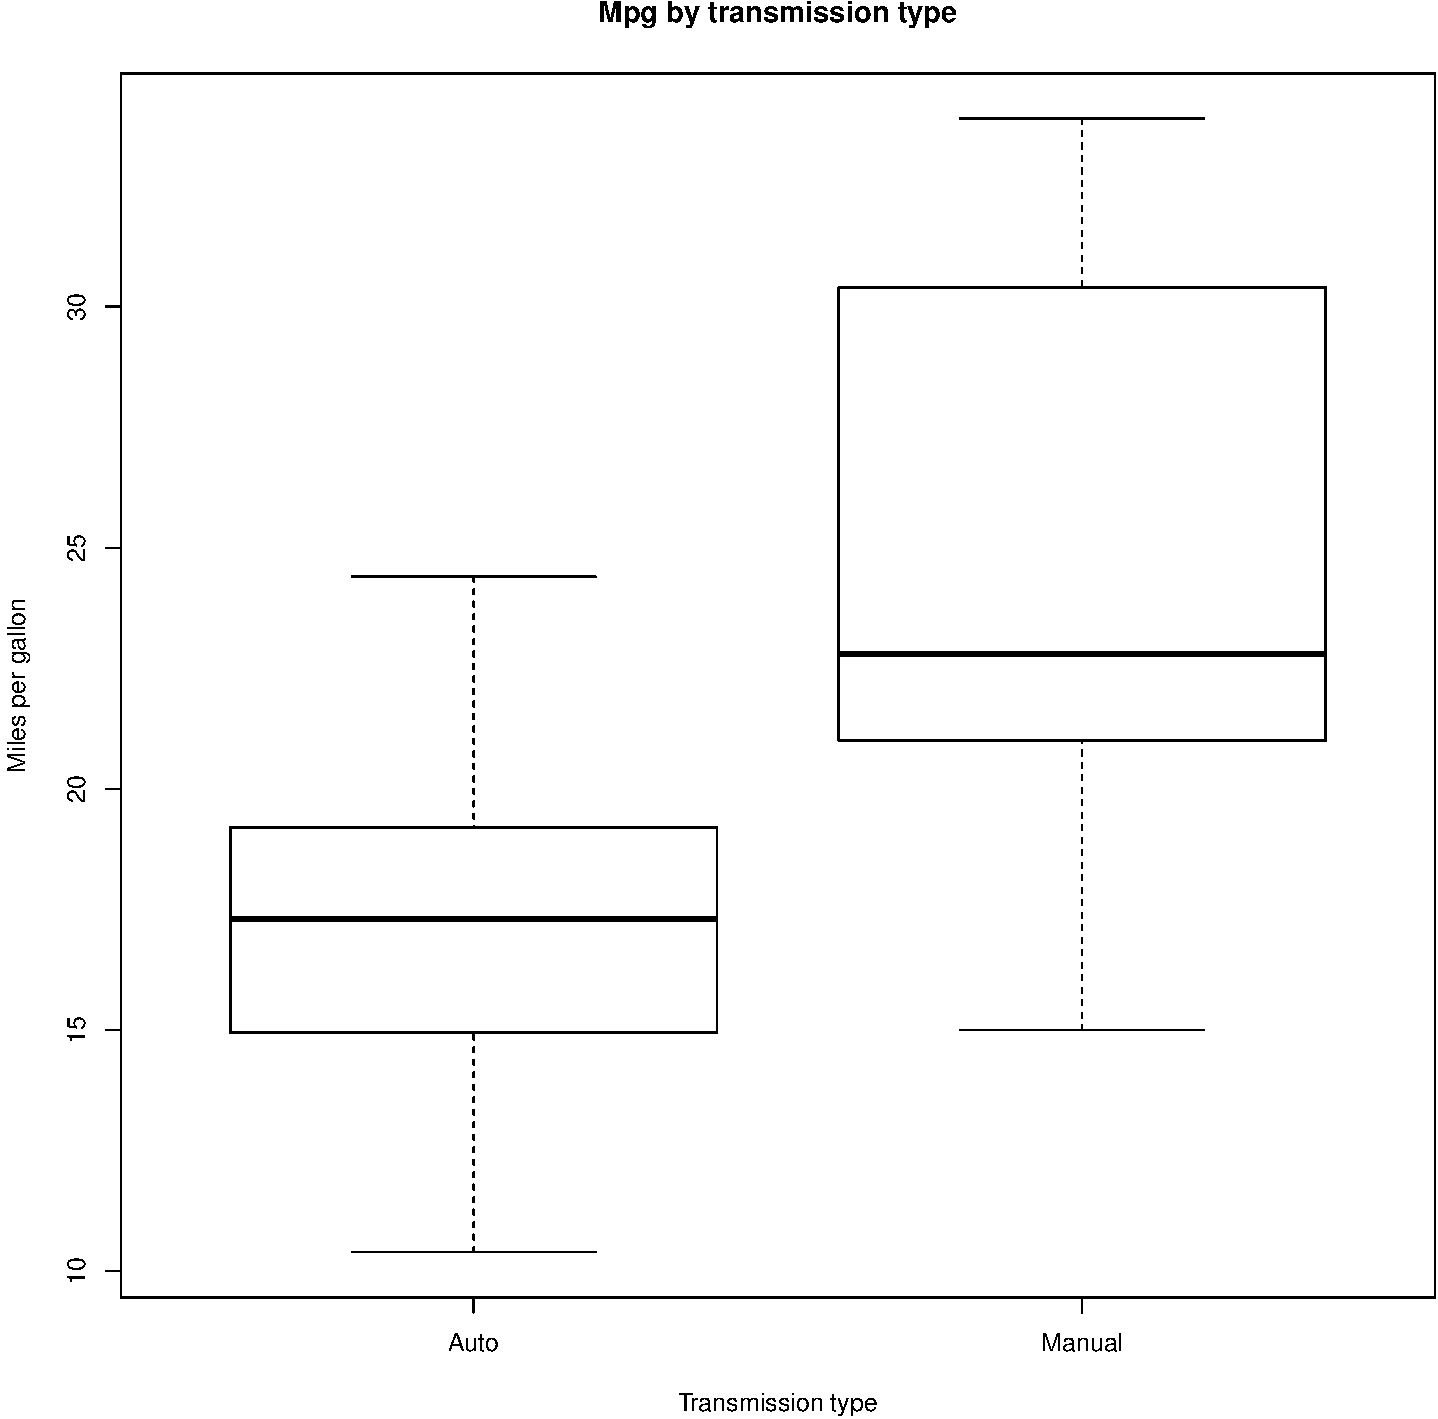
\includegraphics{./Reportbis_files/figure-latex/unnamed-chunk-13.pdf}

\subsubsection{Figure 2 : Pairs graph}\label{figure-2-pairs-graph}

\begin{Shaded}
\begin{Highlighting}[]
\KeywordTok{pairs}\NormalTok{(mtcars, }\DataTypeTok{panel =} \NormalTok{panel.smooth, }\DataTypeTok{main =} \StringTok{"Pairs graph for MTCars"}\NormalTok{)}
\end{Highlighting}
\end{Shaded}

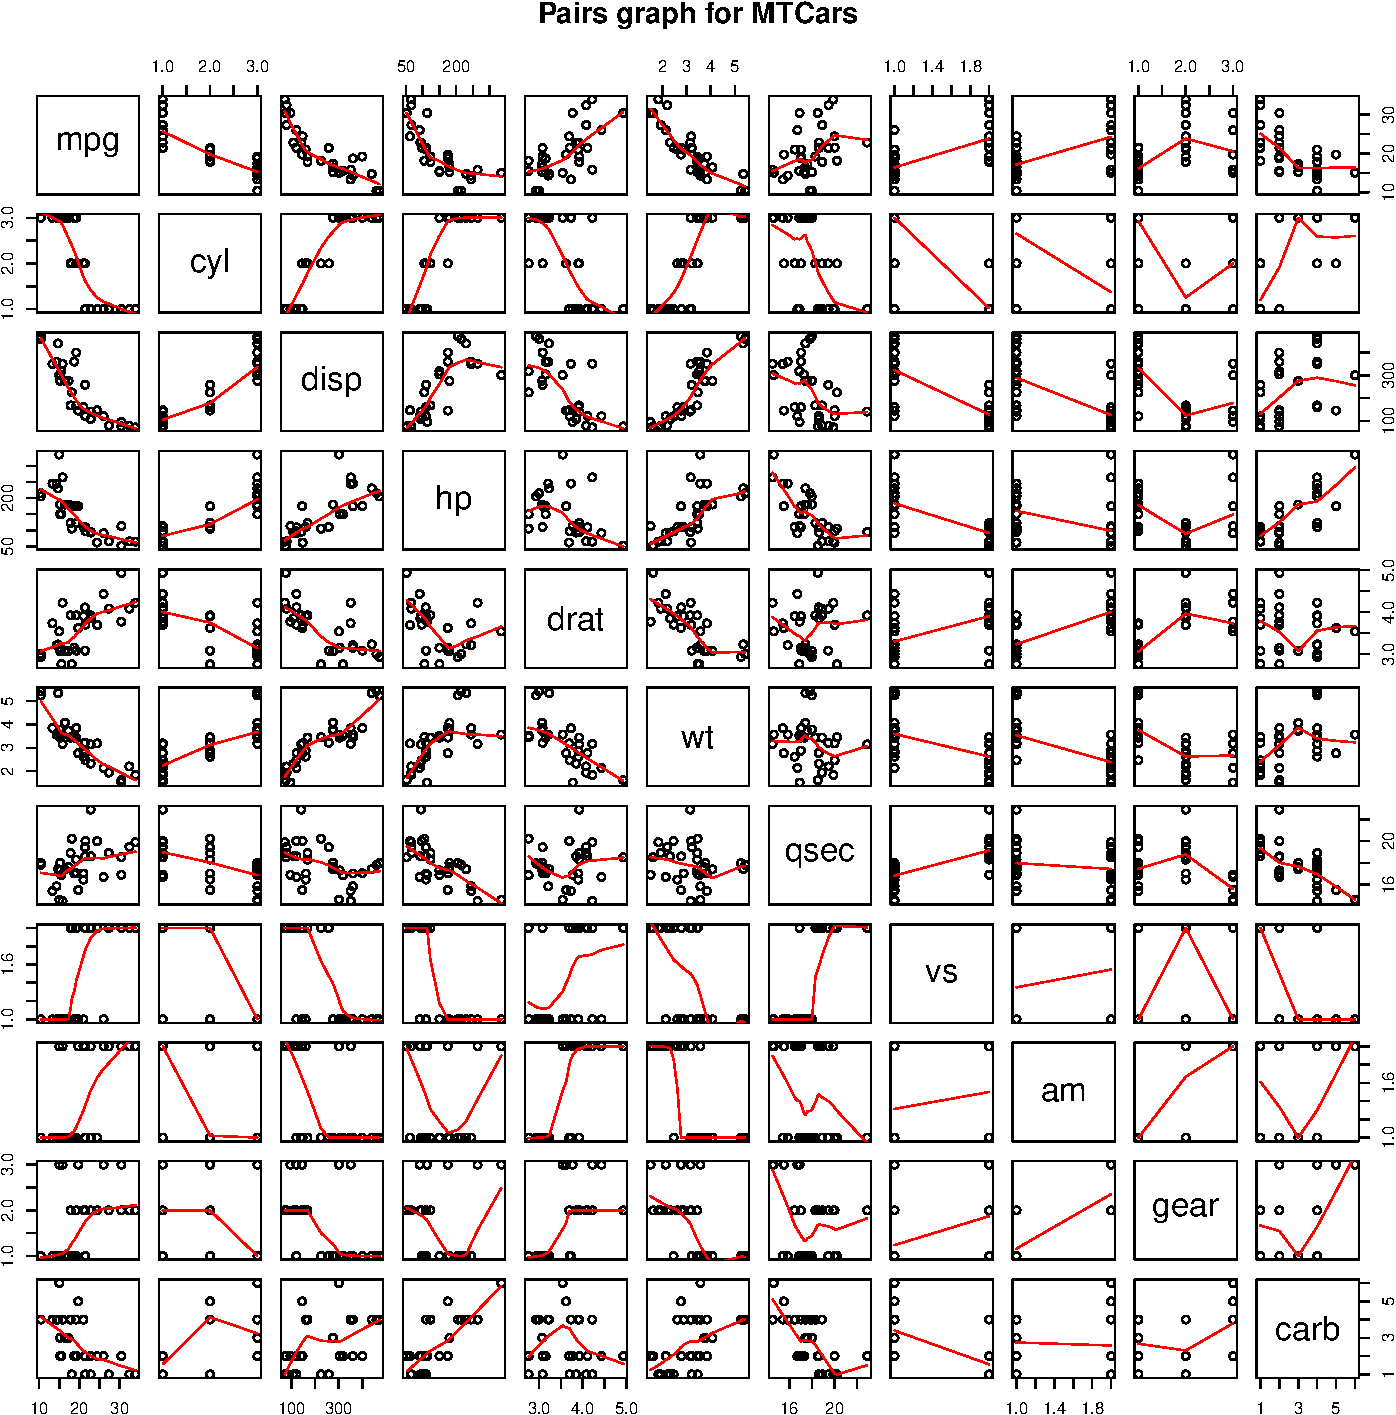
\includegraphics{./Reportbis_files/figure-latex/unnamed-chunk-14.pdf}

\subsubsection{Figure 3 : Residual plots}\label{figure-3-residual-plots}

\begin{Shaded}
\begin{Highlighting}[]
\KeywordTok{par}\NormalTok{(}\DataTypeTok{mfrow =} \KeywordTok{c}\NormalTok{(}\DecValTok{2}\NormalTok{, }\DecValTok{2}\NormalTok{))}
\KeywordTok{plot}\NormalTok{(model)}
\end{Highlighting}
\end{Shaded}

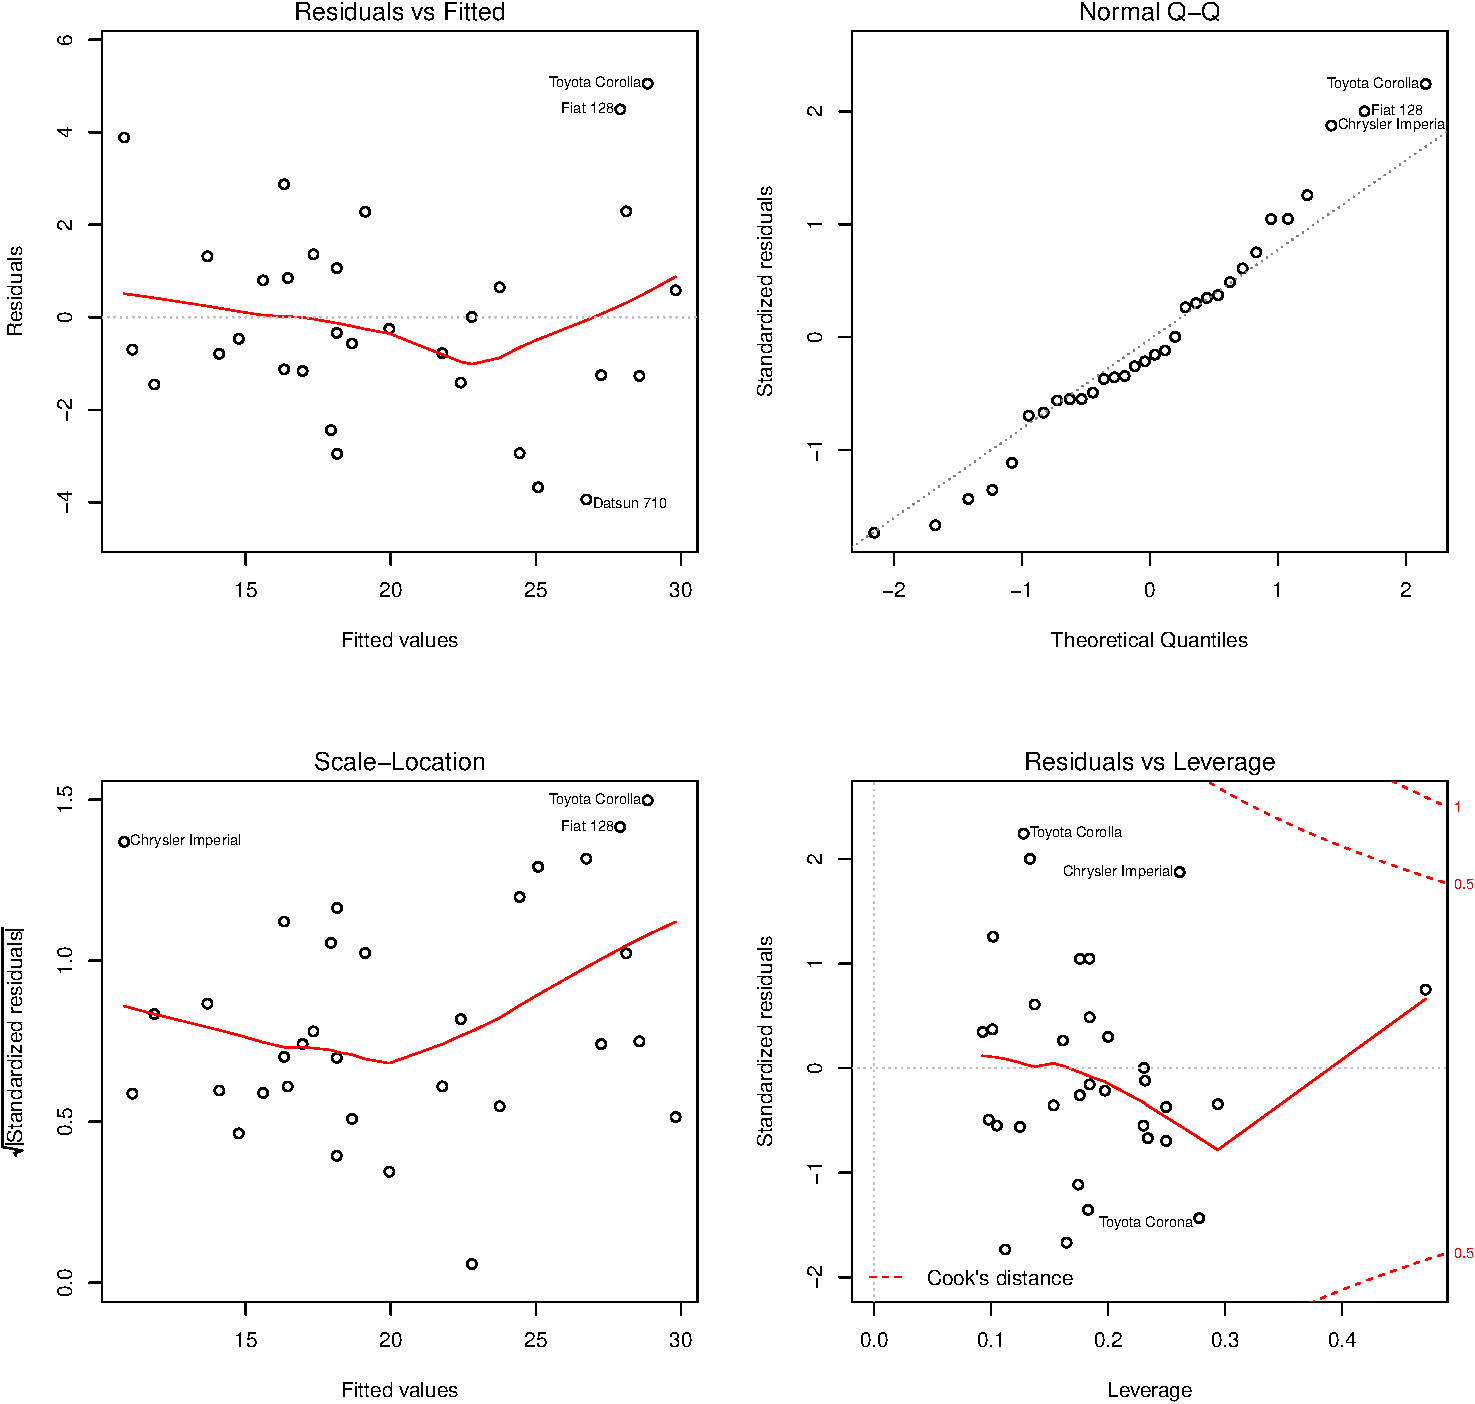
\includegraphics{./Reportbis_files/figure-latex/unnamed-chunk-15.pdf}

\end{document}
